\documentclass[conference]{IEEEtran}
\IEEEoverridecommandlockouts
% The preceding line is only needed to identify funding in the first footnote. If that is unneeded, please comment it out.

\usepackage[backend=biber]{biblatex}
\addbibresource{Article.bib}
\usepackage{amsmath,amssymb,amsfonts}
\usepackage{algorithmic}
\usepackage{graphicx}
\usepackage{textcomp}
\usepackage{xcolor}
\usepackage{hyperref}
\hypersetup{
	urlbordercolor=  0.2 0.8 0.72,
    pdftitle={Linking Gamification, Ludology and Pedagogy: How to Use Serious Games for Various Knowledge Domains},}
\def\BibTeX{{\rm B\kern-.05em{\sc i\kern-.025em b}\kern-.08em
    T\kern-.1667em\lower.7ex\hbox{E}\kern-.125emX}}
\begin{document}

\title{Linking Gamification, Ludology and Pedagogy: How to Use Serious Games for Various Knowledge Domains\\

}

\author{\IEEEauthorblockN{Joshua Esterhuizen}
\IEEEauthorblockA{\textit{School of Computer Science and Information Systems} \\
\textit{North-West University,}\\
Potchefstroom, South Africa \\
\href{mailto:joshua.esterhuizen27@gmail.com}{joshua.esterhuizen27@gmail.com}}
\and

\IEEEauthorblockN{Günther Drevin (Supervisor)}
\IEEEauthorblockA{\textit{School of Computer Science and Information Systems} \\
\textit{North-West University,}\\
Potchefstroom, South Africa \\
\href{mailto:Gunther.Drevin@nwu.ac.za}{Gunther.Drevin@nwu.ac.za}}

}

\maketitle

\begin{abstract}
Education as a whole has seen no major improvements for a long period of time while society has matured and grown rapidly in the same time frame. Due to this teaching and learning methods can be seen as stale to certain students. One way to solve this issue is with the implementation of some from of the technology that has developed over the years. This study looks at the possibility of adapting various domains of knowledge into digital games referred to as Serious Games. The implementation of serious games within teaching may help keep certain students engaged with the content being presented and create further interest in the topic. However, before reaching this stage the means to transform these knowledge domains into a serious games must be studied. This is done by focusing on three fields in particular, those being Gamification, Ludology and Pedagogy.
\end{abstract}

\begin{IEEEkeywords}
Education, Gamification, Knowledge Domains, Ludology, Pedagogy, Serious Games
\end{IEEEkeywords}

\section{Introduction}
Education, as it stands, is still built on a paradigm that is no longer needed in modern society. One major flaw with the current system is that it stifles the creativity and drive of some students as each level of education is largely the same and is, as such, monotonous\cite{Ackoff2008} Therefore, education requires some form of system to create an interest in learning for the students.
\\\\
Ackoff and Greenberg\cite{Ackoff2008} explain that the current traditional means of teaching are no longer as relevant as they once were as it is aimed to produce members of society that were likely to not question any fundamental aspects of how things operated. It is largely a system that focuses on teaching while disregarding learning as the last major stride in development in education was to industrialise it – having them operate efficiently like factories\cite{Ackoff2008}. It is a system that is designed to keep moving often employing a “No Child Left Behind” policy which results in almost no time for anything other than the standardised and constantly measured curriculum\cite{gibson2006games}. 
\\\\
However, with the shift into the “information age”, the requirements of the workforce have also changed. The industrial age being a time of mass-production with the emergence of various new processing technologies and the information age being characterised by the fact that information is being transmitted and generated at an ever-increasing rate due to further technological developments\cite{gibson2006games, Reigeluth1996}. The most notable changes between these ages is that the industrial age focused on conformity and compliance while initiative and diversity - where greater value is placed on each individual’s strengths and contribution to a project or organisation – is the focus of the information age\cite{Reigeluth1996}.  
\\\\
Reigeluth\cite{Reigeluth1996} continues and states that the current paradigm of instruction is not focused on learning but rather categorisation. Ackoff\cite{Ackoff1991} holds a similar viewpoint stating that there is more of a focus on teaching rather than learning. It should be noted that teaching and learning are very distinct from one another as both can take place without the other\cite{Ackoff1991}. Learning is defined as increasing one’s ability to perform an act effectively while trying to meet an objective through acquiring new knowledge whereas teaching is the process of providing this knowledge\cite{Ackoff1991}. Through this, it is clear that institutions under this paradigm aim to give learners a verbose vocabulary to speak on topics that they do not fully comprehend\cite{Ackoff1991}. 
\\\\
Due to this aforementioned paradigm shifts between the ages and in what requirements are desired by most organisations in the information age, a shift in instructional theory is also needed – one such as going from making use of passive learning through traditional teaching means to one that is centred on active learning\cite{Reigeluth1996}.
\\\\
With the recent developments in technology and the fact that technology, in general, is becoming more accessible, some institutions have adopted some forms of digital learning or supplement traditional teaching with digital assistance. Deshpande and Huang\cite{Deshpande2011} state that the current generation of students is the first to grow up with abundant access to technology. They continue to state that, on average, these students spend almost double the time playing video games as they do reading\cite{Deshpande2011}. It can be assumed that from when Deshpande and Huang’s\cite{Deshpande2011} published this work that this figure has increased as with technology and video games as industries. 
\\\\
Virvou, Katsionis and Manos\cite{Virvou2005} echo the point that computer games are popular among individuals who are in schools and as such could provide a means to deliver content in an interesting and engaging manner. 
\\\\
According to Annetta\cite{Annetta2008}, the movement for the inclusion of digital games to be used in teaching and training environments first started in 2003, two years after the field of ludology, the study of games, began to gain traction in academic literature. This initiative is what started the concept of a serious game as one that can be used in an academic sense to relay information. After this point in time, various examples of serious games were made for purely academic study purposes and had found a very large use in simulation for use as explanation aides and medical training.
\\\\
As such, the motivation behind this study is to further investigate the possibility of using video games as a means to encourage learning in teaching environments as current means of teaching may not be optimal for some individuals. This will be accomplished through studying literature in the relevant fields and identifying the instances where it is viable.
 


\section{Literature Review}
\subsection{Serious Games and Ludology}
\subsection{A Pedagogical Approach}
Pedagogy is the filed that deals with the transferal of knowledge in an educational environment through several lenses such as social, political and cultural\cite{Li2012}. As such it encompasses the fields and discussions of instructional design and theory as well as any learning theories – of which several are particularly useful to this study.
\\\\
Learning by doing functions on the principle that skills can be improved through practice and self-perfection on a particular topic or knowledge base\cite{Fisch2009}. This means of instruction has become increasingly popular amongst companies where they are able to make use of “on the job” training as it allows for a person to be productive immediately as well as become more proficient at tasks gradually\cite{Fisch2009}. 
\\\\
The learning by teaching method works under the assumption that learners are able to increase their understanding of a certain topic by teaching it to other learners\cite{Fisch2009}. This method of learning has garnered more usage recently as it is a viable means of learning in environments with too few teachers or instructors and increases the overall learning process\cite{Fisch2009}. Learning methods that place the learner in control are very flexible and as such can be incorporated when attempting to teach various and different fields or subjects\cite{Ackoff1991}. 
\\\\
Gibson et al.\cite{gibson2006games} list and summarise several learning and instructional design theories that have the potential to be applied to a game used for learning. This study will, however, only look at Merrill’s First Principles of Instruction as it is the most recent of the ones depicted  and is one that is very expansive and as such can be used in a variety of manners\cite{gibson2006games}.
\\\\
Before discussing the principles that the name refers to in this theory, Merrill\cite{Merrill2002} provides a few definitions for the terms made use of. A principle in this context is a relationship that is always true regardless of the environment it is applied within – this being the driving factor for deciding to make use of this theory\cite{Merrill2002}. A practice is any instructional activity\cite{Merrill2002}. A program is a means of instruction that makes use of several practices\cite{Merrill2002}. Merrill\cite{Merrill2002} states that the first principles described are able to be implemented in any instructional system or environment as they are “design-oriented” and as such relate more to creating learning environments rather than describing the means of knowledge transfer. Each of the following principles is also accompanied by three “corollaries” each of which Merrill\cite{Merrill2002} likewise explains.
\\\\
The first principle of Merrill’s First Principles of Instruction is that the learning is problem centred. This principle describes three corollaries, the first of which being “Show Task” which states that learners should be shown the types of problems they will be solving or will be able to solve with the knowledge that they attain\cite{Merrill2002}. The next is the “Task Level” which explains that the problems presented should keep learners engaged due to the complexity and not just the action of solving it\cite{Merrill2002}. The last corollary, “Problem Progression” describes that the problems presented should have some form of increasing complexity while still being comparable to the previous iteration of the type of problem\cite{Merrill2002}.
\\\\
The second principle is Activation which means that learning happens whenever previous experiences are used\cite{Merrill2002}. The first corollary, “Previous Experience”, states that the learning process is enhanced when a learner is able to draw upon relevant past experiences and apply the associate knowledge as a foundation for new knowledge\cite{Merrill2002}. “New Knowledge” is the second and explains that learners should be provided with a relevant experience as an additional foundation to add to their knowledge base\cite{Merrill2002}. The last corollary is “Structure” and details that learners should be encouraged to organise new knowledge according to some relevant structure\cite{Merrill2002}.
\\\\
The third principle, Demonstration, proposes that learning takes place when the activities that are undertaken impart the knowledge instead of stating the information\cite{Merrill2002}. “Demonstration Consistency” explains that any examples or visualisation should be kept in line with the original learning goals\cite{Merrill2002}. The next is “Learner Guidance” and states that learners should be shown where the relevant information for problems can be found be it in the form of comparative examples or various representation of one source\cite{Merrill2002}. “Relevant Media” explains that when media is used as a means of demonstration, different types can be used provided that they do not fight for a learner’s attention\cite{Merrill2002}.
\\\\
The fourth principle is Application which states that learning takes place when learners actively solve problems with the new knowledge they have acquired\cite{Merrill2002}. “Practice Consistency” is similar to Demonstration consistency but with a focus on the application of knowledge\cite{Merrill2002}. “Diminishing Coaching” is where the learners are provided with relevant feedback, but it is slowly lessened over time\cite{Merrill2002}. It is also important that the problems provided to learners for practice have a good variety, as explained as “Varied Problems”\cite{Merrill2002}.
\\\\
The fifth, and final, principle is Integration which is when the knowledge a learner has acquired is used by them in their everyday life\cite{Merrill2002}. The first corollary, “Watch Me”, explains that learners are provided to showcase the new knowledge or skill they have acquired\cite{Merrill2002}. “Reflection” deals with giving learners time to be able to debate with others on the topic involved\cite{Merrill2002}. Lastly, “Creation” states that learners should be able to make use of their new knowledge or skill in some personal capacity\cite{Merrill2002}.
\\
\begin{figure}[htbp]
\centerline{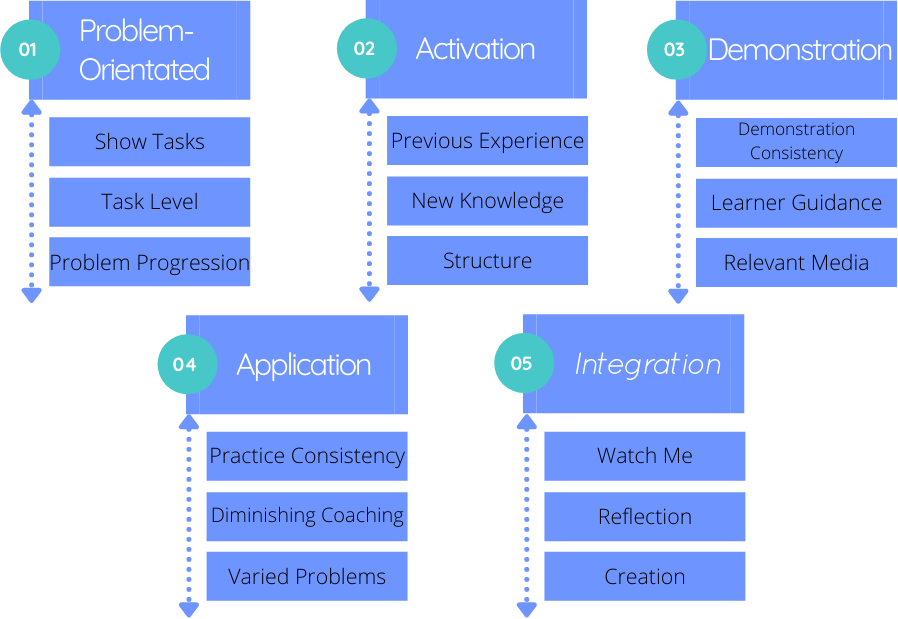
\includegraphics[scale=0.35]{merrill2.png}}
\caption{Own Image summarising Merrill's First Principles}
\label{fig}
\end{figure}
\\
The principles and corollaries provided by Merrill\cite{Merrill2002} provide an expansive and detailed structure to be used when developing any learning opportunity making it an exceptional choice to adapt specifically to a digital game learning system.  It does, however, lack a comprehensive discussion on how to keep learners engaged with the content and, as such, the next subsection will discuss some theories pertaining to the role of motivation in learning.
\\\\
Another important factor to consider is how to keep learners engaged and motivated with the instructional material. One model for motivating learners is the ARCS Model which was developed by John Keller which is frequently referenced in the aforementioned field of instructional design\cite{Kapp2012a}. It is comprised of four main elements with each focusing on designing instruction in a different way\cite{Kapp2012a}. 
\\\\
The first of these is Attention and it is an element that is concerned with gaining and then keeping the learners’ interest. There are three main methods to accomplish this with the first being gaining attention through the use of relatable examples or surprise. The next is to create curiosity within the learners through means such as role-playing or hands-on examples. The last means to keep attention is the variability which means periodically changing the method of delivery\cite{Kapp2012a}.
\\\\
Relevance refers to having the content be relevant to the learner and Kapp\cite{Kapp2012a} mentions that this can be done through orienting the environment around achieving goals, creating a link between the motives of learners and that of the instruction means, displaying that the content is in somewhat familiar to the learners and finally developing a model of the results of learning the presented knowledge.
\\\\
Another element of this model, Confidence, is the expectations of success set by the learner and as such when they meet these expectations they are confident in their ability to do the work\cite{Kapp2012a}. This can be aided by providing learners with clear expectations and requirements upfront about the skill or knowledge. It is also helpful to provide smaller opportunities to succeed as with each success the learners will become more confident\cite{Kapp2012a}.
\\\\
The last element in the ARCS model is Satisfaction and is concerned with giving learners a sense of accomplishment and that the effort in the learning process has some value and weight to it\cite{Kapp2012a}. This can be accomplished by allowing learners to see how their newfound knowledge can be used, either through the use of a real-world demonstration or via some form of simulation\cite{Kapp2012a}.



\subsection{Gamification and the Knowledge Domains}

\section{Methodology}
The following steps were taken to determine how serious games can be used for the various knowledge domains:

\begin{itemize}
\item[1.] Literature surrounding the applicable fields was researched
\item[2.] Case studies concerning serious games was studied and similarities noted
\item[3.] Select theories that aid this process were pinpointed
\item[4.] From this research, recommendations for the knowledge domains were made
\end{itemize}

\subsection{Sampling of Literature}
\subsection{Collection of Case Studies and Determine Similarities}
\subsection{Pinpointing Connected Theories}
\subsection{Extrapolate to other Knowledge Domains}

\section{Findings}
\subsection{Helpful Teaching Theories}
\subsection{Case Studies and the Similarities in Design Principles}

\section{Synthesis from Research}
\subsection{Recommendations per Knowledge Domain}
\subsection{Limitations and Future Research}

\printbibliography

%%------------------------------------------------------------
\subsection{Maintaining the Integrity of the Specifications}

The IEEEtran class file is used to format your paper and style the text. All margins, 
column widths, line spaces, and text fonts are prescribed; please do not 
alter them. You may note peculiarities. For example, the head margin
measures proportionately more than is customary. This measurement 
and others are deliberate, using specifications that anticipate your paper 
as one part of the entire proceedings, and not as an independent document. 
Please do not revise any of the current designations.

\section{Prepare Your Paper Before Styling}
Before you begin to format your paper, first write and save the content as a 
separate text file. Complete all content and organizational editing before 
formatting. Please note sections \ref{AA}--\ref{SCM} below for more information on 
proofreading, spelling and grammar.

Keep your text and graphic files separate until after the text has been 
formatted and styled. Do not number text heads---{\LaTeX} will do that 
for you.

\subsection{Abbreviations and Acronyms}\label{AA}
Define abbreviations and acronyms the first time they are used in the text, 
even after they have been defined in the abstract. Abbreviations such as 
IEEE, SI, MKS, CGS, ac, dc, and rms do not have to be defined. Do not use 
abbreviations in the title or heads unless they are unavoidable.

\subsection{Units}
\begin{itemize}
\item Use either SI (MKS) or CGS as primary units. (SI units are encouraged.) English units may be used as secondary units (in parentheses). An exception would be the use of English units as identifiers in trade, such as ``3.5-inch disk drive''.
\item Avoid combining SI and CGS units, such as current in amperes and magnetic field in oersteds. This often leads to confusion because equations do not balance dimensionally. If you must use mixed units, clearly state the units for each quantity that you use in an equation.
\item Do not mix complete spellings and abbreviations of units: ``Wb/m\textsuperscript{2}'' or ``webers per square meter'', not ``webers/m\textsuperscript{2}''. Spell out units when they appear in text: ``. . . a few henries'', not ``. . . a few H''.
\item Use a zero before decimal points: ``0.25'', not ``.25''. Use ``cm\textsuperscript{3}'', not ``cc''.)
\end{itemize}

\subsection{Equations}
Number equations consecutively. To make your 
equations more compact, you may use the solidus (~/~), the exp function, or 
appropriate exponents. Italicize Roman symbols for quantities and variables, 
but not Greek symbols. Use a long dash rather than a hyphen for a minus 
sign. Punctuate equations with commas or periods when they are part of a 
sentence, as in:
\begin{equation}
a+b=\gamma\label{eq}
\end{equation}

Be sure that the 
symbols in your equation have been defined before or immediately following 
the equation. Use ``\eqref{eq}'', not ``Eq.~\eqref{eq}'' or ``equation \eqref{eq}'', except at 
the beginning of a sentence: ``Equation \eqref{eq} is . . .''

\subsection{\LaTeX-Specific Advice}

Please use ``soft'' (e.g., \verb|\eqref{Eq}|) cross references instead
of ``hard'' references (e.g., \verb|(1)|). That will make it possible
to combine sections, add equations, or change the order of figures or
citations without having to go through the file line by line.

Please don't use the \verb|{eqnarray}| equation environment. Use
\verb|{align}| or \verb|{IEEEeqnarray}| instead. The \verb|{eqnarray}|
environment leaves unsightly spaces around relation symbols.

Please note that the \verb|{subequations}| environment in {\LaTeX}
will increment the main equation counter even when there are no
equation numbers displayed. If you forget that, you might write an
article in which the equation numbers skip from (17) to (20), causing
the copy editors to wonder if you've discovered a new method of
counting.

{\BibTeX} does not work by magic. It doesn't get the bibliographic
data from thin air but from .bib files. If you use {\BibTeX} to produce a
bibliography you must send the .bib files. 

{\LaTeX} can't read your mind. If you assign the same label to a
subsubsection and a table, you might find that Table I has been cross
referenced as Table IV-B3. 

{\LaTeX} does not have precognitive abilities. If you put a
\verb|\label| command before the command that updates the counter it's
supposed to be using, the label will pick up the last counter to be
cross referenced instead. In particular, a \verb|\label| command
should not go before the caption of a figure or a table.

Do not use \verb|\nonumber| inside the \verb|{array}| environment. It
will not stop equation numbers inside \verb|{array}| (there won't be
any anyway) and it might stop a wanted equation number in the
surrounding equation.

\subsection{Some Common Mistakes}\label{SCM}
\begin{itemize}
\item The word ``data'' is plural, not singular.
\item The subscript for the permeability of vacuum $\mu_{0}$, and other common scientific constants, is zero with subscript formatting, not a lowercase letter ``o''.
\item In American English, commas, semicolons, periods, question and exclamation marks are located within quotation marks only when a complete thought or name is cited, such as a title or full quotation. When quotation marks are used, instead of a bold or italic typeface, to highlight a word or phrase, punctuation should appear outside of the quotation marks. A parenthetical phrase or statement at the end of a sentence is punctuated outside of the closing parenthesis (like this). (A parenthetical sentence is punctuated within the parentheses.)
\item A graph within a graph is an ``inset'', not an ``insert''. The word alternatively is preferred to the word ``alternately'' (unless you really mean something that alternates).
\item Do not use the word ``essentially'' to mean ``approximately'' or ``effectively''.
\item In your paper title, if the words ``that uses'' can accurately replace the word ``using'', capitalize the ``u''; if not, keep using lower-cased.
\item Be aware of the different meanings of the homophones ``affect'' and ``effect'', ``complement'' and ``compliment'', ``discreet'' and ``discrete'', ``principal'' and ``principle''.
\item Do not confuse ``imply'' and ``infer''.
\item The prefix ``non'' is not a word; it should be joined to the word it modifies, usually without a hyphen.
\item There is no period after the ``et'' in the Latin abbreviation ``et al.''.
\item The abbreviation ``i.e.'' means ``that is'', and the abbreviation ``e.g.'' means ``for example''.
\end{itemize}
An excellent style manual for science writers is \cite{b7}.

\subsection{Authors and Affiliations}
\textbf{The class file is designed for, but not limited to, six authors.} A 
minimum of one author is required for all conference articles. Author names 
should be listed starting from left to right and then moving down to the 
next line. This is the author sequence that will be used in future citations 
and by indexing services. Names should not be listed in columns nor group by 
affiliation. Please keep your affiliations as succinct as possible (for 
example, do not differentiate among departments of the same organization).

\subsection{Identify the Headings}
Headings, or heads, are organizational devices that guide the reader through 
your paper. There are two types: component heads and text heads.

Component heads identify the different components of your paper and are not 
topically subordinate to each other. Examples include Acknowledgments and 
References and, for these, the correct style to use is ``Heading 5''. Use 
``figure caption'' for your Figure captions, and ``table head'' for your 
table title. Run-in heads, such as ``Abstract'', will require you to apply a 
style (in this case, italic) in addition to the style provided by the drop 
down menu to differentiate the head from the text.

Text heads organize the topics on a relational, hierarchical basis. For 
example, the paper title is the primary text head because all subsequent 
material relates and elaborates on this one topic. If there are two or more 
sub-topics, the next level head (uppercase Roman numerals) should be used 
and, conversely, if there are not at least two sub-topics, then no subheads 
should be introduced.

\subsection{Figures and Tables}
\paragraph{Positioning Figures and Tables} Place figures and tables at the top and 
bottom of columns. Avoid placing them in the middle of columns. Large 
figures and tables may span across both columns. Figure captions should be 
below the figures; table heads should appear above the tables. Insert 
figures and tables after they are cited in the text. Use the abbreviation 
``Fig.~\ref{fig}'', even at the beginning of a sentence.

\begin{table}[htbp]
\caption{Table Type Styles}
\begin{center}
\begin{tabular}{|c|c|c|c|}
\hline
\textbf{Table}&\multicolumn{3}{|c|}{\textbf{Table Column Head}} \\
\cline{2-4} 
\textbf{Head} & \textbf{\textit{Table column subhead}}& \textbf{\textit{Subhead}}& \textbf{\textit{Subhead}} \\
\hline
copy& More table copy$^{\mathrm{a}}$& &  \\
\hline
\multicolumn{4}{l}{$^{\mathrm{a}}$Sample of a Table footnote.}
\end{tabular}
\label{tab1}
\end{center}
\end{table}

\begin{figure}[htbp]
\centerline{
\includegraphics{fig1.png}}
\caption{Example of a figure caption.}
\label{fig}
\end{figure}

Figure Labels: Use 8 point Times New Roman for Figure labels. Use words 
rather than symbols or abbreviations when writing Figure axis labels to 
avoid confusing the reader. As an example, write the quantity 
``Magnetization'', or ``Magnetization, M'', not just ``M''. If including 
units in the label, present them within parentheses. Do not label axes only 
with units. In the example, write ``Magnetization (A/m)'' or ``Magnetization 
\{A[m(1)]\}'', not just ``A/m''. Do not label axes with a ratio of 
quantities and units. For example, write ``Temperature (K)'', not 
``Temperature/K''.

\section*{Acknowledgment}

The preferred spelling of the word ``acknowledgment'' in America is without 
an ``e'' after the ``g''. Avoid the stilted expression ``one of us (R. B. 
G.) thanks $\ldots$''. Instead, try ``R. B. G. thanks$\ldots$''. Put sponsor 
acknowledgments in the unnumbered footnote on the first page.

\section*{References}

Please number citations consecutively within brackets \cite{b1}. The 
sentence punctuation follows the bracket \cite{b2}. Refer simply to the reference 
number, as in \cite{b3}---do not use ``Ref. \cite{b3}'' or ``reference \cite{b3}'' except at 
the beginning of a sentence: ``Reference \cite{b3} was the first $\ldots$''

Number footnotes separately in superscripts. Place the actual footnote at 
the bottom of the column in which it was cited. Do not put footnotes in the 
abstract or reference list. Use letters for table footnotes.

Unless there are six authors or more give all authors' names; do not use 
``et al.''. Papers that have not been published, even if they have been 
submitted for publication, should be cited as ``unpublished'' \cite{b4}. Papers 
that have been accepted for publication should be cited as ``in press'' \cite{b5}. 
Capitalize only the first word in a paper title, except for proper nouns and 
element symbols.

For papers published in translation journals, please give the English 
citation first, followed by the original foreign-language citation \cite{b6}.

\begin{thebibliography}{00}
\bibitem{b1} G. Eason, B. Noble, and I. N. Sneddon, ``On certain integrals of Lipschitz-Hankel type involving products of Bessel functions,'' Phil. Trans. Roy. Soc. London, vol. A247, pp. 529--551, April 1955.
\bibitem{b2} J. Clerk Maxwell, A Treatise on Electricity and Magnetism, 3rd ed., vol. 2. Oxford: Clarendon, 1892, pp.68--73.
\bibitem{b3} I. S. Jacobs and C. P. Bean, ``Fine particles, thin films and exchange anisotropy,'' in Magnetism, vol. III, G. T. Rado and H. Suhl, Eds. New York: Academic, 1963, pp. 271--350.
\bibitem{b4} K. Elissa, ``Title of paper if known,'' unpublished.
\bibitem{b5} R. Nicole, ``Title of paper with only first word capitalized,'' J. Name Stand. Abbrev., in press.
\bibitem{b6} Y. Yorozu, M. Hirano, K. Oka, and Y. Tagawa, ``Electron spectroscopy studies on magneto-optical media and plastic substrate interface,'' IEEE Transl. J. Magn. Japan, vol. 2, pp. 740--741, August 1987 [Digests 9th Annual Conf. Magnetics Japan, p. 301, 1982].
\bibitem{b7} M. Young, The Technical Writer's Handbook. Mill Valley, CA: University Science, 1989.
\end{thebibliography}
\vspace{12pt}
\color{red}
IEEE conference templates contain guidance text for composing and formatting conference papers. Please ensure that all template text is removed from your conference paper prior to submission to the conference. Failure to remove the template text from your paper may result in your paper not being published.
%%-------------------------------------------------------------------

\end{document}
